\section{Economic performance, costs and failure mechanisms}\label{sec:section-08}

The controlled portfolio comparisons do not establish an economic advantage: every primary-block interval below crosses zero after matching the same outer dates and execution rules. Each fold starts a fresh account; the study averages daily active returns across those blocks, not a fictitious continuously invested equity path across the intervening gaps. Approximate detectable daily active effects range from 0.0420\% to 0.0736\%. These are large relative to the registered practical threshold. The bootstrap conditions on the observed outer blocks and cannot establish robustness to an unseen market regime.

\noindent Table~\ref{tab:12} reports controlled daily active returns versus equal weight; primary date-block inference.

\begin{table}[!htbp]\centering\footnotesize\setlength{\tabcolsep}{3pt}\renewcommand{\arraystretch}{1.14}
\caption{Controlled daily active returns versus equal weight; primary date-block inference}\label{tab:12}
\begin{tabular}{@{}>{\raggedright\arraybackslash}p{\dimexpr 0.20312\textwidth-5.000pt\relax}>{\raggedleft\arraybackslash}p{\dimexpr 0.15234\textwidth-5.000pt\relax}>{\raggedleft\arraybackslash}p{\dimexpr 0.18750\textwidth-5.000pt\relax}>{\raggedleft\arraybackslash}p{\dimexpr 0.15234\textwidth-5.000pt\relax}>{\raggedleft\arraybackslash}p{\dimexpr 0.15234\textwidth-5.000pt\relax}>{\raggedleft\arraybackslash}p{\dimexpr 0.15234\textwidth-5.000pt\relax}@{}}
\toprule
\textbf{Policy} & \textbf{Dates} & \textbf{Daily effect} & \textbf{CI low} & \textbf{CI high} & \textbf{Holm p} \\
\midrule
linear & 252 & -0.04\% & -0.08\% & 0.01\% & 0.972 \\
tree & 252 & -0.00\% & -0.05\% & 0.04\% & 1.000 \\
raw & 252 & -0.02\% & -0.06\% & 0.02\% & 1.000 \\
calibrated & 252 & -0.03\% & -0.08\% & 0.02\% & 1.000 \\
fixed\_\allowbreak{}mix & 252 & -0.01\% & -0.05\% & 0.02\% & 1.000 \\
same\_\allowbreak{}gate & 252 & -0.01\% & -0.04\% & 0.02\% & 1.000 \\
separate\_\allowbreak{}gate & 252 & -0.00\% & -0.03\% & 0.03\% & 1.000 \\
trend & 252 & -0.00\% & -0.03\% & 0.03\% & 1.000 \\
\bottomrule\end{tabular}\par\smallskip
\raggedright\textit{Source:} \path{data/research-v2/tables/exp_economic_contrasts.csv}.
\end{table}


For the newly matched audit accounts, each policy begins with 10,000.00 dollars. The adaptive hybrid ends at 9,954.29 dollars and the equal-weight control at 10,254.73 dollars. Hybrid net return is -0.46\%, maximum drawdown -2.21\%, and average gross exposure 55.63\%. These fresh-capital results differ from the sealed continuous-account audit because startup holdings and entry financing differ. The continuous curves below retain their original account history and are labeled accordingly.

\noindent Table~\ref{tab:13} reports fresh-capital audit accounts; zero-rate Sharpe and modeled per-side costs.

\begin{table}[!htbp]\centering\footnotesize\setlength{\tabcolsep}{3pt}\renewcommand{\arraystretch}{1.14}
\caption{Fresh-capital audit accounts; zero-rate Sharpe and modeled per-side costs}\label{tab:13}
\begin{tabular}{@{}>{\raggedright\arraybackslash}p{\dimexpr 0.20339\textwidth-5.143pt\relax}>{\raggedleft\arraybackslash}p{\dimexpr 0.13559\textwidth-5.143pt\relax}>{\raggedleft\arraybackslash}p{\dimexpr 0.13220\textwidth-5.143pt\relax}>{\raggedleft\arraybackslash}p{\dimexpr 0.13220\textwidth-5.143pt\relax}>{\raggedleft\arraybackslash}p{\dimexpr 0.13220\textwidth-5.143pt\relax}>{\raggedleft\arraybackslash}p{\dimexpr 0.13220\textwidth-5.143pt\relax}>{\raggedleft\arraybackslash}p{\dimexpr 0.13220\textwidth-5.143pt\relax}@{}}
\toprule
\textbf{Policy} & \textbf{Net return} & \textbf{Sharpe} & \textbf{Max DD} & \textbf{Exposure} & \textbf{Costs (\$)} & \textbf{Fills} \\
\midrule
trend & -0.48\% & -0.328 & -2.34\% & 56.67\% & 15.24 & 184 \\
ml & -0.48\% & -0.360 & -2.13\% & 32.22\% & 29.57 & 119 \\
adaptive\_\allowbreak{}hybrid & -0.46\% & -0.309 & -2.21\% & 55.63\% & 20.51 & 217 \\
equal\_\allowbreak{}weight & 2.55\% & 1.297 & -2.66\% & 74.45\% & 13.58 & 205 \\
cash & 0.00\% & - & 0.00\% & 0.00\% & 0.00 & 0 \\
\bottomrule\end{tabular}\par\smallskip
\raggedright\textit{Source:} \path{data/research-v2/tables/diag_portfolio.csv}.
\end{table}


\noindent Figure~\ref{fig:10} shows continuous accounts from their original common start; these are not fresh audit allocations.

\begin{figure}[htbp]\centering
% Native editable figure; frozen statistics 0d291b4aebf8c524dc6705d872c070feb990e86a1cebbd59a758f400b240c952
\begin{tikzpicture}\begin{groupplot}[group style={group size=1 by 3,vertical sep=9mm},width=.90\linewidth,height=4.1cm,scaled y ticks=false,y tick label style={/pgf/number format/fixed,/pgf/number format/precision=2},xmin=0,xmax=685,xtick={0,125,251,376,502,625,685},xticklabels={Jan24,Jul24,Jan25,Jul25,Jan26,Jul26,Sep26}]
\nextgroupplot[ylabel={Equity (USD)},legend columns=3,legend style={at={(.5,1.06)},anchor=south},xticklabels=\empty]
\addplot+[blue,mark=none,thin] table[col sep=comma,x=session_index,y=equity] {data/portfolio-trend.csv};
\addlegendentry{trend}
\addplot+[orange,mark=none,thin] table[col sep=comma,x=session_index,y=equity] {data/portfolio-ml.csv};
\addlegendentry{ml}
\addplot+[teal,mark=none,thin] table[col sep=comma,x=session_index,y=equity] {data/portfolio-adaptive_hybrid.csv};
\addlegendentry{adaptive\_hybrid}
\addplot+[black,mark=none,thin] table[col sep=comma,x=session_index,y=equity] {data/portfolio-equal_weight.csv};
\addlegendentry{equal\_weight}
\addplot+[gray,mark=none,thin] table[col sep=comma,x=session_index,y=equity] {data/portfolio-cash.csv};
\addlegendentry{cash}
\nextgroupplot[ylabel={Drawdown (fraction)},xticklabels=\empty]
\addplot+[blue,mark=none,thin] table[col sep=comma,x=session_index,y=drawdown] {data/portfolio-trend.csv};
\addplot+[orange,mark=none,thin] table[col sep=comma,x=session_index,y=drawdown] {data/portfolio-ml.csv};
\addplot+[teal,mark=none,thin] table[col sep=comma,x=session_index,y=drawdown] {data/portfolio-adaptive_hybrid.csv};
\addplot+[black,mark=none,thin] table[col sep=comma,x=session_index,y=drawdown] {data/portfolio-equal_weight.csv};
\addplot+[gray,mark=none,thin] table[col sep=comma,x=session_index,y=drawdown] {data/portfolio-cash.csv};
\nextgroupplot[ylabel={Gross exposure}]
\addplot+[blue,mark=none,thin] table[col sep=comma,x=session_index,y=exposure] {data/portfolio-trend.csv};
\addplot+[orange,mark=none,thin] table[col sep=comma,x=session_index,y=exposure] {data/portfolio-ml.csv};
\addplot+[teal,mark=none,thin] table[col sep=comma,x=session_index,y=exposure] {data/portfolio-adaptive_hybrid.csv};
\addplot+[black,mark=none,thin] table[col sep=comma,x=session_index,y=exposure] {data/portfolio-equal_weight.csv};
\addplot+[gray,mark=none,thin] table[col sep=comma,x=session_index,y=exposure] {data/portfolio-cash.csv};
\end{groupplot}\end{tikzpicture}
\caption{Continuous accounts from their original common start; these are not fresh audit allocations.}\label{fig:10}
\end{figure}

\noindent Figure~\ref{fig:11} shows recorded exposure, turnover and cost diagnostics under the shared ledger contract.

\begin{figure}[htbp]\centering
% Native editable figure; frozen statistics 0d291b4aebf8c524dc6705d872c070feb990e86a1cebbd59a758f400b240c952
\begin{minipage}[t]{.48\linewidth}\centering
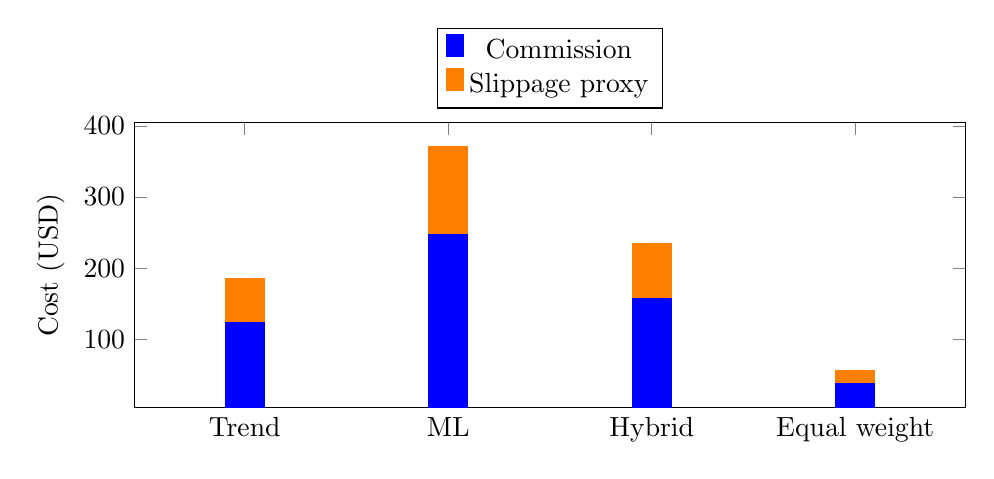
\begin{tikzpicture}
\begin{axis}[width=\linewidth,height=5.2cm,xtick={0,1,2,3},xticklabels={Trend,ML,Hybrid,Equal weight},enlarge x limits=.18,ybar stacked,bar width=14pt,ylabel={Cost (USD)},legend style={at={(.5,1.05)},anchor=south}]
\addplot+[blue] coordinates {(0,123.207203497) (1,247.34447747) (2,156.536969368) (3,37.1132402528)};
\addlegendentry{Commission}
\addplot+[orange] coordinates {(0,61.6036017484) (1,123.672238735) (2,78.2684846841) (3,18.5566201264)};
\addlegendentry{Slippage proxy}

\end{axis}
\end{tikzpicture}
\end{minipage}
\hfill
\begin{minipage}[t]{.48\linewidth}\centering
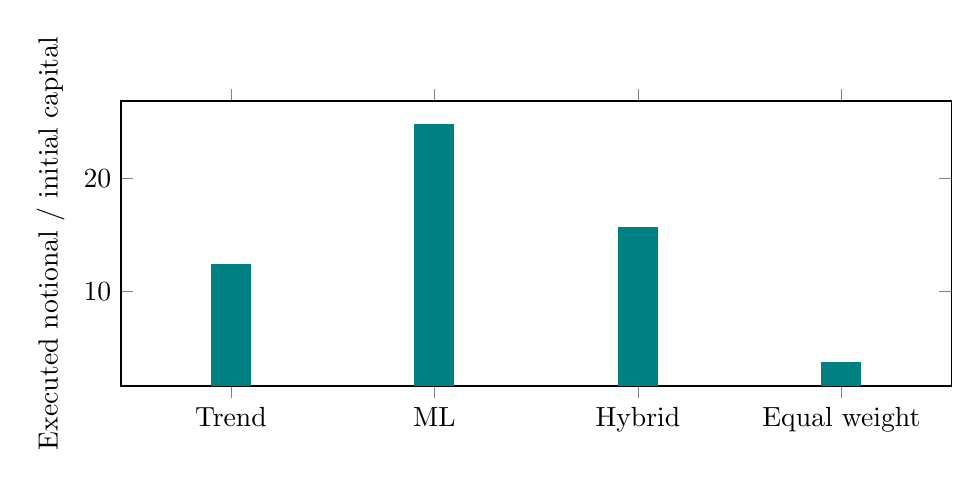
\begin{tikzpicture}
\begin{axis}[width=\linewidth,height=5.2cm,xtick={0,1,2,3},xticklabels={Trend,ML,Hybrid,Equal weight},enlarge x limits=.18,ybar,bar width=14pt,ylabel={Executed notional / initial capital}]
\addplot+[teal] coordinates {(0,12.3207203497) (1,24.734447747) (2,15.6536969368) (3,3.71132402528)};
\end{axis}
\end{tikzpicture}
\end{minipage}
\caption{Recorded exposure, turnover and cost diagnostics under the shared ledger contract.}\label{fig:11}
\end{figure}

Prediction loss and portfolio return need not rank models identically. The trading rule uses estimated payoff magnitude, abstention, weekly decisions and constrained capital. A prediction can be directionally wrong while its account is in cash; a correct signal can still lose after a delayed fill or costs. The decomposition therefore examines exposure, turnover, fill rejections, realized net outcomes and open holdings rather than attributing every equity change to classifier accuracy.

Over the full continuous hybrid account, modeled combined costs are 234.81 dollars across 2,541 fills. There are 1,367 sell fills, which include partial reductions rather than necessarily completed flat-to-flat episodes. Their net realized profit is 2,929.53 dollars; open holdings and unclosed costs still matter for total equity. The 86 completed position episodes have a 46.51\% win rate, materially different from the sell-fill statistic. Neither is a strategy's independent trade success probability. The completed-position episode table reconciles closed net profit and terminal open-position profit to total account profit, preventing partial sales from being counted as independent completed trades.

\noindent Table~\ref{tab:14} reports hybrid closed-position episodes versus still-open positions.

\begin{table}[!htbp]\centering\footnotesize\setlength{\tabcolsep}{3pt}\renewcommand{\arraystretch}{1.14}
\caption{Hybrid closed-position episodes versus still-open positions}\label{tab:14}
\begin{tabular}{@{}>{\raggedright\arraybackslash}p{\dimexpr 0.12303\textwidth-5.143pt\relax}>{\raggedleft\arraybackslash}p{\dimexpr 0.12303\textwidth-5.143pt\relax}>{\raggedleft\arraybackslash}p{\dimexpr 0.12303\textwidth-5.143pt\relax}>{\raggedleft\arraybackslash}p{\dimexpr 0.13880\textwidth-5.143pt\relax}>{\raggedleft\arraybackslash}p{\dimexpr 0.17666\textwidth-5.143pt\relax}>{\raggedleft\arraybackslash}p{\dimexpr 0.15142\textwidth-5.143pt\relax}>{\raggedleft\arraybackslash}p{\dimexpr 0.16404\textwidth-5.143pt\relax}@{}}
\toprule
\textbf{Period} & \textbf{Closed} & \textbf{Open} & \textbf{Closed wins} & \textbf{Closed P\&L (\$)} & \textbf{Open P\&L (\$)} & \textbf{Total P\&L (\$)} \\
\midrule
full & 86 & 18 & 46.51\% & 1605.17 & 1902.90 & 3508.07 \\
audit & 14 & 16 & 14.29\% & -141.85 & 96.14 & -45.71 \\
\bottomrule\end{tabular}\par\smallskip
\raggedright\textit{Source:} \path{data/research-v2/tables/diag_round_trip_summary.csv}.
\end{table}


\noindent Table~\ref{tab:15} reports largest audit hybrid forecast losses, selected by registered loss ranking.

\begin{table}[!htbp]\centering\footnotesize\setlength{\tabcolsep}{3pt}\renewcommand{\arraystretch}{1.14}
\caption{Largest audit hybrid forecast losses, selected by registered loss ranking}\label{tab:15}
\begin{tabular}{@{}>{\raggedright\arraybackslash}p{\dimexpr 0.13176\textwidth-5.000pt\relax}>{\raggedright\arraybackslash}p{\dimexpr 0.33784\textwidth-5.000pt\relax}>{\raggedright\arraybackslash}p{\dimexpr 0.13176\textwidth-5.000pt\relax}>{\raggedright\arraybackslash}p{\dimexpr 0.13176\textwidth-5.000pt\relax}>{\raggedleft\arraybackslash}p{\dimexpr 0.13514\textwidth-5.000pt\relax}>{\raggedleft\arraybackslash}p{\dimexpr 0.13176\textwidth-5.000pt\relax}@{}}
\toprule
\textbf{Symbol} & \textbf{Decision} & \textbf{Observed} & \textbf{Predicted} & \textbf{Confidence} & \textbf{Loss} \\
\midrule
TSLA & 2026-09-09 00:00:00+00:00 & FLAT & UP & 0.547 & 2.612 \\
TSLA & 2026-09-10 00:00:00+00:00 & FLAT & UP & 0.487 & 2.528 \\
GOOGL & 2026-07-30 00:00:00+00:00 & FLAT & UP & 0.468 & 2.321 \\
XLI & 2026-08-20 00:00:00+00:00 & DOWN & UP & 0.638 & 2.154 \\
DIA & 2026-08-12 00:00:00+00:00 & DOWN & FLAT & 0.514 & 2.113 \\
\bottomrule\end{tabular}\par\smallskip
\raggedright\textit{Source:} \path{data/research-v2/tables/diag_failures.csv}.
\end{table}


The reported failure cases follow registered selection rules: representative observations, the largest confident forecast errors and the largest adverse account contributions. They are not handpicked success stories. A loss concentration can reveal concentrated exposure or a difficult period, but explaining why a model produced a probability requires tracing its actual inputs and fitted state. Descriptive associations between a gate and losses are not causal gate benefits. Component and gate interventions provide the relevant controlled evidence.

Across the registered completed hybrid sensitivity scenarios, the lowest terminal return is -1.17\% in delay\_1; the highest is 0.93\% in reserve\_zero. These extrema are descriptive stress outcomes, not candidates selected for deployment. A rejected-order scenario can improve a realized sample by avoiding losing exposure, and a temporary gap can worsen drawdown without changing the terminal price. Both effects require examining the full path, fills and rejections, not just ending wealth.

\noindent Table~\ref{tab:16} reports hybrid execution and risk sensitivities; fresh-capital audit.

\begin{table}[!htbp]\centering\footnotesize\setlength{\tabcolsep}{3pt}\renewcommand{\arraystretch}{1.14}
\caption{Hybrid execution and risk sensitivities; fresh-capital audit}\label{tab:16}
\begin{tabular}{@{}>{\raggedright\arraybackslash}p{\dimexpr 0.20189\textwidth-5.000pt\relax}>{\raggedright\arraybackslash}p{\dimexpr 0.30284\textwidth-5.000pt\relax}>{\raggedleft\arraybackslash}p{\dimexpr 0.12618\textwidth-5.000pt\relax}>{\raggedleft\arraybackslash}p{\dimexpr 0.12303\textwidth-5.000pt\relax}>{\raggedleft\arraybackslash}p{\dimexpr 0.12303\textwidth-5.000pt\relax}>{\raggedleft\arraybackslash}p{\dimexpr 0.12303\textwidth-5.000pt\relax}@{}}
\toprule
\textbf{Scenario} & \textbf{Status} & \textbf{Net return} & \textbf{Max DD} & \textbf{Fills} & \textbf{Rejected} \\
\midrule
base & completed & -0.46\% & -2.21\% & 217 & 6 \\
cost\_\allowbreak{}zero & completed & -0.25\% & -2.17\% & 217 & 6 \\
cost\_\allowbreak{}2x & completed & -0.66\% & -2.26\% & 217 & 6 \\
cost\_\allowbreak{}4x & completed & -1.07\% & -2.35\% & 217 & 6 \\
delay\_\allowbreak{}1 & completed & -1.17\% & -2.29\% & 219 & 4 \\
liquidity\_\allowbreak{}50pct & completed & -0.35\% & -2.22\% & 1,043 & 25 \\
gap\_\allowbreak{}down\_\allowbreak{}10pct & completed & -0.46\% & -6.45\% & 217 & 6 \\
risk\_\allowbreak{}gross\_\allowbreak{}60pct & completed & -0.47\% & -2.09\% & 213 & 7 \\
reserve\_\allowbreak{}zero & completed & 0.93\% & -2.09\% & 151 & 70 \\
missing\_\allowbreak{}bar & expected\_\allowbreak{}validation\_\allowbreak{}halt & - & - & - & - \\
\bottomrule\end{tabular}\par\smallskip
\raggedright\textit{Source:} \path{data/research-v2/tables/diag_stress.csv}.
\end{table}


\noindent Figure~\ref{fig:12} shows registered execution sensitivities; terminal return and path risk answer different questions.

\begin{figure}[htbp]\centering
% Native editable figure; frozen statistics 0d291b4aebf8c524dc6705d872c070feb990e86a1cebbd59a758f400b240c952
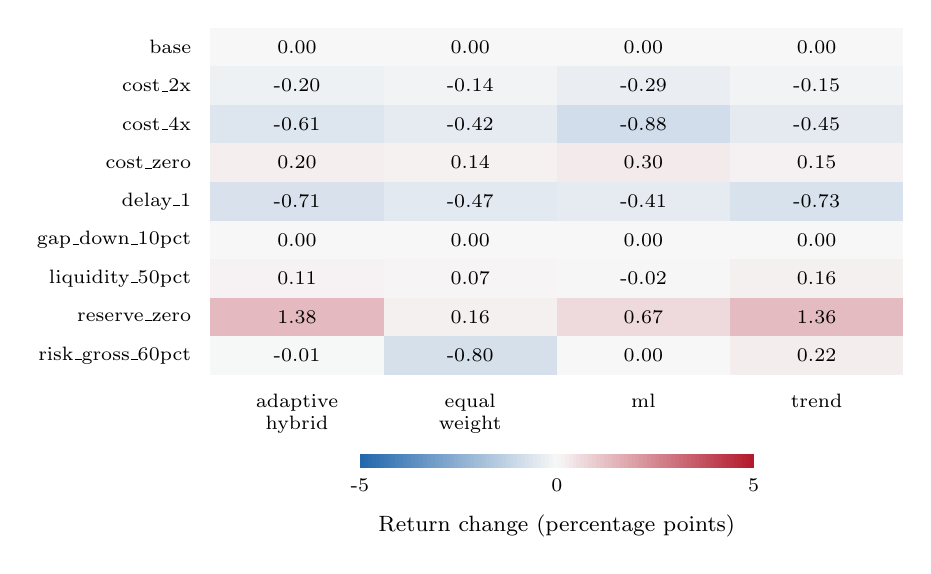
\begin{tikzpicture}[x=1cm,y=1cm,font=\scriptsize]
\node[anchor=east] at (-.12,4.165) {base};
\fill[fill={rgb,255:red,247;green,247;blue,247}] (0,3.92) rectangle ++(2.2,0.49);
\node at (1.1,4.165) {0.00};
\fill[fill={rgb,255:red,247;green,247;blue,247}] (2.2,3.92) rectangle ++(2.2,0.49);
\node at (3.3,4.165) {0.00};
\fill[fill={rgb,255:red,247;green,247;blue,247}] (4.4,3.92) rectangle ++(2.2,0.49);
\node at (5.5,4.165) {0.00};
\fill[fill={rgb,255:red,247;green,247;blue,247}] (6.6,3.92) rectangle ++(2.2,0.49);
\node at (7.7,4.165) {0.00};
\node[anchor=east] at (-.12,3.675) {cost\_2x};
\fill[fill={rgb,255:red,238;green,241;blue,244}] (0,3.43) rectangle ++(2.2,0.49);
\node at (1.1,3.675) {-0.20};
\fill[fill={rgb,255:red,241;green,243;blue,245}] (2.2,3.43) rectangle ++(2.2,0.49);
\node at (3.3,3.675) {-0.14};
\fill[fill={rgb,255:red,234;green,238;blue,243}] (4.4,3.43) rectangle ++(2.2,0.49);
\node at (5.5,3.675) {-0.29};
\fill[fill={rgb,255:red,241;green,243;blue,245}] (6.6,3.43) rectangle ++(2.2,0.49);
\node at (7.7,3.675) {-0.15};
\node[anchor=east] at (-.12,3.185) {cost\_4x};
\fill[fill={rgb,255:red,221;green,229;blue,238}] (0,2.94) rectangle ++(2.2,0.49);
\node at (1.1,3.185) {-0.61};
\fill[fill={rgb,255:red,229;green,235;blue,241}] (2.2,2.94) rectangle ++(2.2,0.49);
\node at (3.3,3.185) {-0.42};
\fill[fill={rgb,255:red,209;green,221;blue,234}] (4.4,2.94) rectangle ++(2.2,0.49);
\node at (5.5,3.185) {-0.88};
\fill[fill={rgb,255:red,228;green,234;blue,240}] (6.6,2.94) rectangle ++(2.2,0.49);
\node at (7.7,3.185) {-0.45};
\node[anchor=east] at (-.12,2.695) {cost\_zero};
\fill[fill={rgb,255:red,244;green,238;blue,239}] (0,2.45) rectangle ++(2.2,0.49);
\node at (1.1,2.695) {0.20};
\fill[fill={rgb,255:red,245;green,241;blue,241}] (2.2,2.45) rectangle ++(2.2,0.49);
\node at (3.3,2.695) {0.14};
\fill[fill={rgb,255:red,243;green,234;blue,235}] (4.4,2.45) rectangle ++(2.2,0.49);
\node at (5.5,2.695) {0.30};
\fill[fill={rgb,255:red,245;green,240;blue,241}] (6.6,2.45) rectangle ++(2.2,0.49);
\node at (7.7,2.695) {0.15};
\node[anchor=east] at (-.12,2.205) {delay\_1};
\fill[fill={rgb,255:red,217;green,226;blue,236}] (0,1.96) rectangle ++(2.2,0.49);
\node at (1.1,2.205) {-0.71};
\fill[fill={rgb,255:red,227;green,233;blue,240}] (2.2,1.96) rectangle ++(2.2,0.49);
\node at (3.3,2.205) {-0.47};
\fill[fill={rgb,255:red,229;green,235;blue,241}] (4.4,1.96) rectangle ++(2.2,0.49);
\node at (5.5,2.205) {-0.41};
\fill[fill={rgb,255:red,216;green,226;blue,236}] (6.6,1.96) rectangle ++(2.2,0.49);
\node at (7.7,2.205) {-0.73};
\node[anchor=east] at (-.12,1.715) {gap\_down\_10pct};
\fill[fill={rgb,255:red,247;green,247;blue,247}] (0,1.47) rectangle ++(2.2,0.49);
\node at (1.1,1.715) {0.00};
\fill[fill={rgb,255:red,247;green,247;blue,247}] (2.2,1.47) rectangle ++(2.2,0.49);
\node at (3.3,1.715) {0.00};
\fill[fill={rgb,255:red,247;green,247;blue,247}] (4.4,1.47) rectangle ++(2.2,0.49);
\node at (5.5,1.715) {0.00};
\fill[fill={rgb,255:red,247;green,247;blue,247}] (6.6,1.47) rectangle ++(2.2,0.49);
\node at (7.7,1.715) {0.00};
\node[anchor=east] at (-.12,1.225) {liquidity\_50pct};
\fill[fill={rgb,255:red,246;green,242;blue,243}] (0,0.98) rectangle ++(2.2,0.49);
\node at (1.1,1.225) {0.11};
\fill[fill={rgb,255:red,246;green,244;blue,244}] (2.2,0.98) rectangle ++(2.2,0.49);
\node at (3.3,1.225) {0.07};
\fill[fill={rgb,255:red,246;green,246;blue,247}] (4.4,0.98) rectangle ++(2.2,0.49);
\node at (5.5,1.225) {-0.02};
\fill[fill={rgb,255:red,245;green,240;blue,240}] (6.6,0.98) rectangle ++(2.2,0.49);
\node at (7.7,1.225) {0.16};
\node[anchor=east] at (-.12,0.735) {reserve\_zero};
\fill[fill={rgb,255:red,228;green,185;blue,191}] (0,0.49) rectangle ++(2.2,0.49);
\node at (1.1,0.735) {1.38};
\fill[fill={rgb,255:red,245;green,240;blue,240}] (2.2,0.49) rectangle ++(2.2,0.49);
\node at (3.3,0.735) {0.16};
\fill[fill={rgb,255:red,238;green,217;blue,220}] (4.4,0.49) rectangle ++(2.2,0.49);
\node at (5.5,0.735) {0.67};
\fill[fill={rgb,255:red,228;green,187;blue,192}] (6.6,0.49) rectangle ++(2.2,0.49);
\node at (7.7,0.735) {1.36};
\node[anchor=east] at (-.12,0.245) {risk\_gross\_60pct};
\fill[fill={rgb,255:red,246;green,247;blue,247}] (0,0) rectangle ++(2.2,0.49);
\node at (1.1,0.245) {-0.01};
\fill[fill={rgb,255:red,213;green,224;blue,235}] (2.2,0) rectangle ++(2.2,0.49);
\node at (3.3,0.245) {-0.80};
\fill[fill={rgb,255:red,247;green,247;blue,247}] (4.4,0) rectangle ++(2.2,0.49);
\node at (5.5,0.245) {0.00};
\fill[fill={rgb,255:red,244;green,237;blue,238}] (6.6,0) rectangle ++(2.2,0.49);
\node at (7.7,0.245) {0.22};
\node[anchor=north,align=center] at (1.1,-.12) {adaptive\\hybrid};
\node[anchor=north,align=center] at (3.3,-.12) {equal\\weight};
\node[anchor=north,align=center] at (5.5,-.12) {ml};
\node[anchor=north,align=center] at (7.7,-.12) {trend};
\fill[fill={rgb,255:red,35;green,103;blue,173}] (1.9,-1.18) rectangle ++(.051,.18);
\fill[fill={rgb,255:red,39;green,106;blue,174}] (1.95,-1.18) rectangle ++(.051,.18);
\fill[fill={rgb,255:red,44;green,109;blue,176}] (2,-1.18) rectangle ++(.051,.18);
\fill[fill={rgb,255:red,48;green,112;blue,177}] (2.05,-1.18) rectangle ++(.051,.18);
\fill[fill={rgb,255:red,52;green,115;blue,179}] (2.1,-1.18) rectangle ++(.051,.18);
\fill[fill={rgb,255:red,57;green,118;blue,180}] (2.15,-1.18) rectangle ++(.051,.18);
\fill[fill={rgb,255:red,61;green,121;blue,182}] (2.2,-1.18) rectangle ++(.051,.18);
\fill[fill={rgb,255:red,65;green,124;blue,183}] (2.25,-1.18) rectangle ++(.051,.18);
\fill[fill={rgb,255:red,69;green,127;blue,185}] (2.3,-1.18) rectangle ++(.051,.18);
\fill[fill={rgb,255:red,74;green,130;blue,186}] (2.35,-1.18) rectangle ++(.051,.18);
\fill[fill={rgb,255:red,78;green,132;blue,188}] (2.4,-1.18) rectangle ++(.051,.18);
\fill[fill={rgb,255:red,82;green,135;blue,189}] (2.45,-1.18) rectangle ++(.051,.18);
\fill[fill={rgb,255:red,86;green,138;blue,191}] (2.5,-1.18) rectangle ++(.051,.18);
\fill[fill={rgb,255:red,91;green,141;blue,192}] (2.55,-1.18) rectangle ++(.051,.18);
\fill[fill={rgb,255:red,95;green,144;blue,194}] (2.6,-1.18) rectangle ++(.051,.18);
\fill[fill={rgb,255:red,99;green,147;blue,195}] (2.65,-1.18) rectangle ++(.051,.18);
\fill[fill={rgb,255:red,104;green,150;blue,197}] (2.7,-1.18) rectangle ++(.051,.18);
\fill[fill={rgb,255:red,108;green,153;blue,198}] (2.75,-1.18) rectangle ++(.051,.18);
\fill[fill={rgb,255:red,112;green,156;blue,200}] (2.8,-1.18) rectangle ++(.051,.18);
\fill[fill={rgb,255:red,116;green,159;blue,201}] (2.85,-1.18) rectangle ++(.051,.18);
\fill[fill={rgb,255:red,121;green,161;blue,203}] (2.9,-1.18) rectangle ++(.051,.18);
\fill[fill={rgb,255:red,125;green,164;blue,204}] (2.95,-1.18) rectangle ++(.051,.18);
\fill[fill={rgb,255:red,129;green,167;blue,206}] (3,-1.18) rectangle ++(.051,.18);
\fill[fill={rgb,255:red,134;green,170;blue,207}] (3.05,-1.18) rectangle ++(.051,.18);
\fill[fill={rgb,255:red,138;green,173;blue,209}] (3.1,-1.18) rectangle ++(.051,.18);
\fill[fill={rgb,255:red,142;green,176;blue,210}] (3.15,-1.18) rectangle ++(.051,.18);
\fill[fill={rgb,255:red,146;green,179;blue,212}] (3.2,-1.18) rectangle ++(.051,.18);
\fill[fill={rgb,255:red,151;green,182;blue,213}] (3.25,-1.18) rectangle ++(.051,.18);
\fill[fill={rgb,255:red,155;green,185;blue,215}] (3.3,-1.18) rectangle ++(.051,.18);
\fill[fill={rgb,255:red,159;green,188;blue,216}] (3.35,-1.18) rectangle ++(.051,.18);
\fill[fill={rgb,255:red,164;green,190;blue,218}] (3.4,-1.18) rectangle ++(.051,.18);
\fill[fill={rgb,255:red,168;green,193;blue,219}] (3.45,-1.18) rectangle ++(.051,.18);
\fill[fill={rgb,255:red,172;green,196;blue,221}] (3.5,-1.18) rectangle ++(.051,.18);
\fill[fill={rgb,255:red,176;green,199;blue,222}] (3.55,-1.18) rectangle ++(.051,.18);
\fill[fill={rgb,255:red,181;green,202;blue,224}] (3.6,-1.18) rectangle ++(.051,.18);
\fill[fill={rgb,255:red,185;green,205;blue,225}] (3.65,-1.18) rectangle ++(.051,.18);
\fill[fill={rgb,255:red,189;green,208;blue,227}] (3.7,-1.18) rectangle ++(.051,.18);
\fill[fill={rgb,255:red,194;green,211;blue,228}] (3.75,-1.18) rectangle ++(.051,.18);
\fill[fill={rgb,255:red,198;green,214;blue,230}] (3.8,-1.18) rectangle ++(.051,.18);
\fill[fill={rgb,255:red,202;green,217;blue,231}] (3.85,-1.18) rectangle ++(.051,.18);
\fill[fill={rgb,255:red,206;green,219;blue,233}] (3.9,-1.18) rectangle ++(.051,.18);
\fill[fill={rgb,255:red,211;green,222;blue,234}] (3.95,-1.18) rectangle ++(.051,.18);
\fill[fill={rgb,255:red,215;green,225;blue,236}] (4,-1.18) rectangle ++(.051,.18);
\fill[fill={rgb,255:red,219;green,228;blue,237}] (4.05,-1.18) rectangle ++(.051,.18);
\fill[fill={rgb,255:red,223;green,231;blue,239}] (4.1,-1.18) rectangle ++(.051,.18);
\fill[fill={rgb,255:red,228;green,234;blue,240}] (4.15,-1.18) rectangle ++(.051,.18);
\fill[fill={rgb,255:red,232;green,237;blue,242}] (4.2,-1.18) rectangle ++(.051,.18);
\fill[fill={rgb,255:red,236;green,240;blue,243}] (4.25,-1.18) rectangle ++(.051,.18);
\fill[fill={rgb,255:red,241;green,243;blue,245}] (4.3,-1.18) rectangle ++(.051,.18);
\fill[fill={rgb,255:red,245;green,246;blue,246}] (4.35,-1.18) rectangle ++(.051,.18);
\fill[fill={rgb,255:red,246;green,245;blue,245}] (4.4,-1.18) rectangle ++(.051,.18);
\fill[fill={rgb,255:red,245;green,240;blue,241}] (4.45,-1.18) rectangle ++(.051,.18);
\fill[fill={rgb,255:red,244;green,236;blue,237}] (4.5,-1.18) rectangle ++(.051,.18);
\fill[fill={rgb,255:red,242;green,231;blue,233}] (4.55,-1.18) rectangle ++(.051,.18);
\fill[fill={rgb,255:red,241;green,227;blue,229}] (4.6,-1.18) rectangle ++(.051,.18);
\fill[fill={rgb,255:red,239;green,222;blue,225}] (4.65,-1.18) rectangle ++(.051,.18);
\fill[fill={rgb,255:red,238;green,218;blue,220}] (4.7,-1.18) rectangle ++(.051,.18);
\fill[fill={rgb,255:red,237;green,214;blue,216}] (4.75,-1.18) rectangle ++(.051,.18);
\fill[fill={rgb,255:red,235;green,209;blue,212}] (4.8,-1.18) rectangle ++(.051,.18);
\fill[fill={rgb,255:red,234;green,205;blue,208}] (4.85,-1.18) rectangle ++(.051,.18);
\fill[fill={rgb,255:red,233;green,200;blue,204}] (4.9,-1.18) rectangle ++(.051,.18);
\fill[fill={rgb,255:red,231;green,196;blue,200}] (4.95,-1.18) rectangle ++(.051,.18);
\fill[fill={rgb,255:red,230;green,191;blue,196}] (5,-1.18) rectangle ++(.051,.18);
\fill[fill={rgb,255:red,228;green,187;blue,192}] (5.05,-1.18) rectangle ++(.051,.18);
\fill[fill={rgb,255:red,227;green,182;blue,188}] (5.1,-1.18) rectangle ++(.051,.18);
\fill[fill={rgb,255:red,226;green,178;blue,184}] (5.15,-1.18) rectangle ++(.051,.18);
\fill[fill={rgb,255:red,224;green,173;blue,180}] (5.2,-1.18) rectangle ++(.051,.18);
\fill[fill={rgb,255:red,223;green,169;blue,176}] (5.25,-1.18) rectangle ++(.051,.18);
\fill[fill={rgb,255:red,221;green,164;blue,172}] (5.3,-1.18) rectangle ++(.051,.18);
\fill[fill={rgb,255:red,220;green,160;blue,167}] (5.35,-1.18) rectangle ++(.051,.18);
\fill[fill={rgb,255:red,219;green,156;blue,163}] (5.4,-1.18) rectangle ++(.051,.18);
\fill[fill={rgb,255:red,217;green,151;blue,159}] (5.45,-1.18) rectangle ++(.051,.18);
\fill[fill={rgb,255:red,216;green,147;blue,155}] (5.5,-1.18) rectangle ++(.051,.18);
\fill[fill={rgb,255:red,215;green,142;blue,151}] (5.55,-1.18) rectangle ++(.051,.18);
\fill[fill={rgb,255:red,213;green,138;blue,147}] (5.6,-1.18) rectangle ++(.051,.18);
\fill[fill={rgb,255:red,212;green,133;blue,143}] (5.65,-1.18) rectangle ++(.051,.18);
\fill[fill={rgb,255:red,210;green,129;blue,139}] (5.7,-1.18) rectangle ++(.051,.18);
\fill[fill={rgb,255:red,209;green,124;blue,135}] (5.75,-1.18) rectangle ++(.051,.18);
\fill[fill={rgb,255:red,208;green,120;blue,131}] (5.8,-1.18) rectangle ++(.051,.18);
\fill[fill={rgb,255:red,206;green,115;blue,127}] (5.85,-1.18) rectangle ++(.051,.18);
\fill[fill={rgb,255:red,205;green,111;blue,123}] (5.9,-1.18) rectangle ++(.051,.18);
\fill[fill={rgb,255:red,204;green,107;blue,118}] (5.95,-1.18) rectangle ++(.051,.18);
\fill[fill={rgb,255:red,202;green,102;blue,114}] (6,-1.18) rectangle ++(.051,.18);
\fill[fill={rgb,255:red,201;green,98;blue,110}] (6.05,-1.18) rectangle ++(.051,.18);
\fill[fill={rgb,255:red,199;green,93;blue,106}] (6.1,-1.18) rectangle ++(.051,.18);
\fill[fill={rgb,255:red,198;green,89;blue,102}] (6.15,-1.18) rectangle ++(.051,.18);
\fill[fill={rgb,255:red,197;green,84;blue,98}] (6.2,-1.18) rectangle ++(.051,.18);
\fill[fill={rgb,255:red,195;green,80;blue,94}] (6.25,-1.18) rectangle ++(.051,.18);
\fill[fill={rgb,255:red,194;green,75;blue,90}] (6.3,-1.18) rectangle ++(.051,.18);
\fill[fill={rgb,255:red,192;green,71;blue,86}] (6.35,-1.18) rectangle ++(.051,.18);
\fill[fill={rgb,255:red,191;green,66;blue,82}] (6.4,-1.18) rectangle ++(.051,.18);
\fill[fill={rgb,255:red,190;green,62;blue,78}] (6.45,-1.18) rectangle ++(.051,.18);
\fill[fill={rgb,255:red,188;green,57;blue,74}] (6.5,-1.18) rectangle ++(.051,.18);
\fill[fill={rgb,255:red,187;green,53;blue,70}] (6.55,-1.18) rectangle ++(.051,.18);
\fill[fill={rgb,255:red,186;green,49;blue,65}] (6.6,-1.18) rectangle ++(.051,.18);
\fill[fill={rgb,255:red,184;green,44;blue,61}] (6.65,-1.18) rectangle ++(.051,.18);
\fill[fill={rgb,255:red,183;green,40;blue,57}] (6.7,-1.18) rectangle ++(.051,.18);
\fill[fill={rgb,255:red,181;green,35;blue,53}] (6.75,-1.18) rectangle ++(.051,.18);
\fill[fill={rgb,255:red,180;green,31;blue,49}] (6.8,-1.18) rectangle ++(.051,.18);
\fill[fill={rgb,255:red,179;green,26;blue,45}] (6.85,-1.18) rectangle ++(.051,.18);
\node[anchor=north] at (1.9,-1.2) {-5};
\node[anchor=north] at (4.4,-1.2) {0};
\node[anchor=north] at (6.9,-1.2) {5};
\node[anchor=north,font=\footnotesize] at (4.4,-1.65) {Return change (percentage points)};
\end{tikzpicture}
\caption{Registered execution sensitivities; terminal return and path risk answer different questions.}\label{fig:12}
\end{figure}

The simulator's costs are assumptions rather than measured execution. Fixed proportional slippage cannot represent all auction impact, spreads, illiquidity or market halts. Bounded fill scenarios explore one aspect of capacity without certifying real fill quality. A small simulated account may reduce some capacity concerns, but that does not make every close executable at the modeled price. Broker deployment would require timing, corporate-action and reconciliation evidence that this study deliberately does not claim.
